\section{Introduction}\label{sec:intro}

Core decomposition ranks vertices by the amount of cohesive structure that still surrounds them after weak vertices are removed~\cite{kcoreSeidman,coreAlg,communityFinder}.
%
The classical $k$-core uses edges as the witness of cohesion.
%
Many graph mining tasks need a stronger witness, because a group may pass an edge-degree threshold while containing few triangles, $4$-cliques, or larger coordinated patterns.
%
The \emph{$(1,s)$-nucleus decomposition}~\cite{nucleusSariyuce14} gives this vertex-centric higher-order ranking.
%
For a fixed $s$, it assigns each vertex the largest value $k$ for which the vertex belongs to a maximal region where every vertex participates in at least $k$ internal $s$-cliques.
%
At $s=2$, this is the $k$-core.
%
At $s=3$, it ranks vertices by triangle-supported cohesion.
%
At larger $s$, it exposes progressively tighter clique-based kernels.

\begin{figure}[t]
\centering
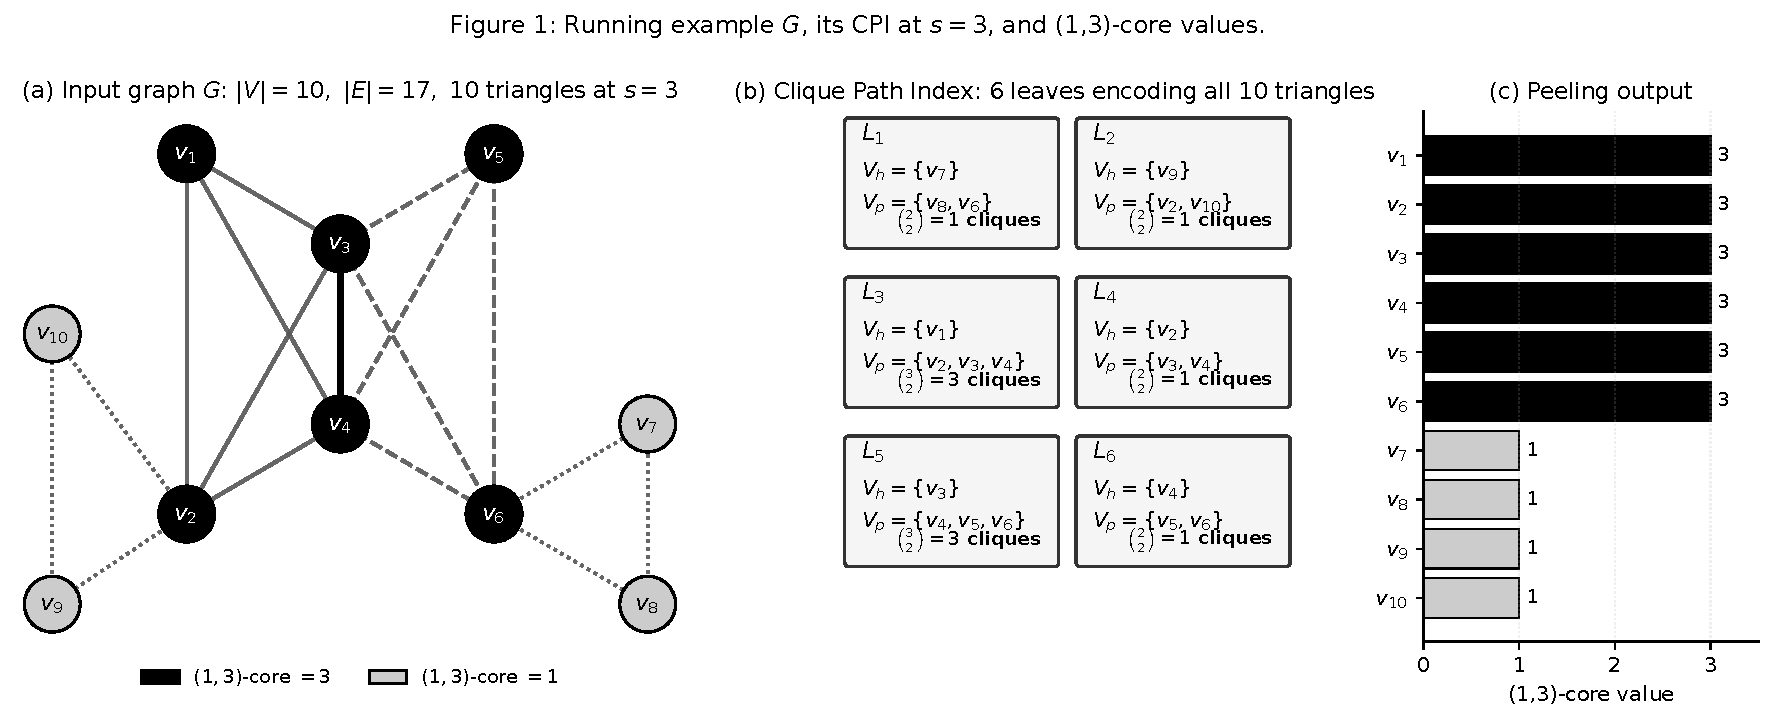
\includegraphics[width=0.7\linewidth]{figures/fig1_overview.pdf}
\caption{Running example of $(1,3)$-nucleus decomposition.}
\Description{Running-example graph topology: 10 vertices, 17 edges, with two K_4 blocks plus two pendant triangles. Node shade indicates (1,3)-core value.}
\label{fig:overview}
\end{figure}

\begin{example}\label{exa:overview}
Figure~\ref{fig:overview} shows a $10$-vertex graph at $s=3$.
%
The six vertices $v_1,\ldots,v_6$ belong to two triangle-rich $K_4$ blocks; each of them participates in at least three triangles supported by other vertices of the same value, so all six have $(1,3)$-core value $3$.
%
The remaining four vertices $v_7,\ldots,v_{10}$ belong to a single pendant triangle, supporting only one triangle each, so all four have $(1,3)$-core value $1$.
%
A formal definition is given in Section~\ref{sec:prelim}; we revisit this graph as a running example throughout the paper.
\end{example}

\stitle{Challenges.}
Computing $(1,s)$-nucleus decomposition at high $s$ is hard because the number of $s$-cliques can be enormous; the current state of the art avoids explicit enumeration with the Clique Path Index, or \cpi{}~\cite{NuclearCD}.
%
A \cpi{} path stores a hold set and a pivot set; it compactly represents all $s$-cliques formed by taking every hold vertex and choosing the remaining vertices from the pivot set.
%
This representation makes general $(r,s)$-nucleus decomposition practical, but using it efficiently for the vertex-centric case $r=1$ raises three challenges.

\sstitle{Residual state during peeling.}
Each peel step must update the surviving support of every remaining vertex.
%
The general $(r,s)$ algorithm achieves this by maintaining the \cpi{} as mutable residual state: it stores per-path vertex sets, a reverse vertex-to-path index, and a priority queue, and rewrites these structures every time a vertex is popped.
%
The challenge is whether this mutability is necessary at $r=1$, where peeling removes vertices but does not delete edges.
%
If not, residual maintenance becomes pure arithmetic over a static incidence layout.

\sstitle{Memory footprint of the residual index.}
The residual structures that support peeling also dominate memory.
%
Per-path vertex hash sets, the reverse vertex-to-path map, and the live Bron--Kerbosch recursion tree together pay constant-factor overhead per vertex--path incidence on top of the clique-encoding cost.
%
The challenge is to encode the same $s$-clique witnesses with a layout whose memory grows with the vertex--path incidence count $\Sig$ alone, so that the achievable $s$ on a fixed-memory machine is dictated by $\Sig$ rather than by hash-table overhead.

\sstitle{Construction as the new bottleneck.}
Once peeling becomes counter-only, the cost profile shifts: on many real graphs the static index takes seconds to minutes to construct while peeling takes milliseconds, so the index builder is the next bottleneck.
%
The challenge is to construct the static \cpi{} in parallel without paying the synchronisation cost that the mutable design requires for path rewrites.

\stitle{State-of-the-Art and Limitations.}
The current state of the art for general $(r,s)$-nucleus decomposition is \cbnd~\cite{NuclearCD}, the mutable-\cpi{} algorithm.
%
\cbnd{} addresses the general case correctly, but inherits three weaknesses when restricted to $r=1$.

\sstitle{Mutable residual-index maintenance.}
\cbnd{} rewrites path records and updates a hash-indexed reverse map at every peel step.
%
This work is intrinsic to the mutable design.
%
Our ablation on $171$ matched cells shows that simply replacing the mutable index with a static one (still using a full-pass solver) already gives a $3.80\times$ geometric-mean peel-time speedup; the residual rewrites are a real cost, not a constant factor.

\sstitle{High memory consumption.}
The residual structures that \cbnd{} must keep mutable in the general $(r,s)$ setting — per-path membership queries, reverse vertex-to-path lookup, and the live recursion tree used to rewrite paths — together cost roughly $88\Sig$ bytes per incidence (Section~\ref{sec:exp}, Table~\ref{tab:mem}), close to an order of magnitude more than what a static encoding of the same witnesses requires.
%
The geometric-mean memory ratio \cbnd{}/\spinStar{} is $1.55\times$ on the matched cells and $3.92\times$ at maximum; on a billion-scale graph the overhead pushes \cbnd{} past the $503$ GB available at every $s$, so the algorithm never completes.

\sstitle{Construction as the residual bottleneck.}
Even after cheap peeling, \cbnd{} pays the full construction cost; on the densest benchmark graph at $s=3$, construction takes about $127$ seconds and peeling takes $351$ milliseconds, so the static index builder dominates total runtime by $360\times$ on this configuration.
%
Without a parallel builder, the end-to-end speedup over \cbnd{} stays at $1.10\times$ on the matched cells even though the peel-time speedup is $13.50\times$.

\stitle{Our Solution and Contributions.}
For $(1,s)$-nucleus decomposition we show that vertex peeling preserves the \cpi{} structure: a set of vertices that formed a clique when the \cpi{} was built remains a clique throughout the peel.
%
A path stops contributing only when one of its hold vertices is removed; otherwise its only dynamic state is an integer counter of how many of its pivots remain.
%
This invariant turns exact decomposition into counter arithmetic over a static incidence layout, which in turn unlocks an incremental peel schedule and a parallel builder.
%
Our contributions address the three challenges one-for-one and add two further pieces that follow from the same static-\cpi{} foundation.

\sstitle{Static-\cpi{} invariant for $(1,s)$ (solves Limitation 1).}
We prove that vertex peeling never rewrites the stored hold or pivot sets (Theorem~\ref{thm:vertex-removal}) and give a closed-form expression for the support loss caused by each path event (Lemma~\ref{lem:support-delta}).
%
The dynamic state of a path collapses to a liveness bit and a single integer counter, so the per-peel residual rewrites disappear and the ablation in RQ7 confirms a $3.80\times$ geometric-mean peel-time speedup over \cbnd{} from this change alone.

\sstitle{Elimination of residual structures (solves Limitation 2).}
A corollary of Theorem~\ref{thm:vertex-removal} is that three of \cbnd{}'s residual structures cease to carry information once the invariant is established: (i) the per-path vertex hash sets, because membership in a path is already determined by the path's fixed hold/pivot sets; (ii) the reverse vertex-to-path map, because the vertex-to-path relation is fixed at construction and never edited; and (iii) the mutable Bron--Kerbosch recursion tree, because no path is ever rewritten during peeling.
%
This collapses the per-incidence space cost from $\approx 88\Sig$ bytes to $\approx 10\Sig$ bytes (Table~\ref{tab:mem}); the measured geometric-mean memory ratio \cbnd{}/\spinStar{} is $1.55\times$ over $307$ matched cells, and a billion-scale graph becomes decomposable on a $503$ GB machine on which \cbnd{} cannot start.

\sstitle{Parallel static-\cpi{} construction (solves Limitation 3).}
Because the static-\cpi{} output is invariant under the order in which seed vertices are processed and contains no mutable shared state, seed enumeration partitions into independent subproblems.
%
\paraBuild{} (Algorithm~\ref{alg:parabuild}) constructs the index by running these subproblems in parallel and combining their outputs by a deterministic merge whose result does not depend on the schedule; the empirical scaling reaches $23.4\times$ at $T{=}24$ threads.

The three contributions above address the three limitations one-for-one.
%
Two further contributions follow from the same static-\cpi{} foundation:

\sstitle{Direct and incremental solvers over the static index.}
We formulate \spin{} as the direct threshold-support iteration on \cpi{} witness counts (Algorithm~\ref{alg:localH}) and \spinStar{} as its incremental optimization (Algorithm~\ref{alg:peelH}) that computes the same fixed point in peel order without repeated full-graph passes (Lemma~\ref{lem:equivalence}).
%
\spinStar{} delivers a $36.2\times$ geometric-mean peel-time speedup over \spin{} on $291$ matched cells.

\sstitle{Core-value hierarchy from the static \cpi{}.}
After peeling, each \cpi{} leaf can be treated as a hyperedge born at the minimum core value among its stored vertices.
%
A descending union--find scan over the leaves recovers the $s$-clique-connected super-level join tree in $O(\Sig\log\Sig)$ time without re-enumerating $s$-cliques (Algorithm~\ref{alg:buildhier}); the hierarchy is a byproduct of preserving the \cpi{} rather than a separate decomposition problem.

\sstitle{Comprehensive experimental evaluation.}
We compare against \cbnd{} on ten real-world graphs ($307$ matched configurations, headline peel speedup $13.50\times$ gmean / $44.76\times$ max, memory-usage ratio $1.55\times$ gmean), report phase behaviour and parallel construction, push the pipeline to a billion-scale graph (where \cbnd{} cannot complete), and use case studies to evaluate whether the $r=1$ specialization is practically useful.

The rest of the paper follows this dependency chain.
%
Section~\ref{sec:prelim} defines the problem, the \cpi{}, and the mutable baseline.
%
Section~\ref{sec:static} derives the static-\cpi{} invariant from the vertex-removal rule.
%
Section~\ref{sec:hindex} derives \spin{} and \spinStar{} from the same threshold-support fixed point.
%
Section~\ref{sec:parabuild} parallelizes construction after peeling becomes cheap.
%
Section~\ref{sec:buildhier} extracts the hierarchy from static \cpi{} leaves after peeling.
%
Sections~\ref{sec:exp} and~\ref{sec:casestudy} report performance and application evidence.
%
Sections~\ref{sec:related} and~\ref{sec:conclusion} position and conclude the paper.
